\subsection{Проводники в электрическом поле. Основная задача электростатики. Теорема единственности}

\begin{definition}
    Проводник — вещество или материальное тело, В котором имеются заряды, способные переносить электрический ток, 
    называется проводником. В металлах переносчиками тока служат свободные (не привязанные к атомам) электроны, 
    в электролитах - ионы, в плазме - и электроны, и ионы. Для электростатических явлений поле внутри проводника равно нулю.
\end{definition}

Механизм исчезновения электрического поля в проводниках связан со смещением свободных зарядов ровно настолько, 
чтобы как раз компенсировать внешнее электрическое поле, если таковое имеется. При изменении внешнего поля свободные заряды 
в проводнике перераспределяются, а в момент перераспределения в проводнике течет ток.

\begin{remark}
    Основная задача электростатики.

    Общей задачей расчета электростатического поля является определение напряженности поля во всех его точках по заданным зарядам. 

    Для электростатического поля задача полностью решается отысканием потенциала как функции координат. Обратная задача поиска 
    распределения зарядов по заданной напряженности решается с помощью уравнения Пуассона или с помощью уравнения Лапласа
    и граничного условия у поверхности заряженных проводящих тел. Это наиболее простой тип задач. 

    Однако большей частью задача оказывается значительно сложнее. Обычно рассматривается система заряженных проводящих тел с 
    известной геометрией, окруженных диэлектриком, в котором отсутствуют объемные заряды. Заданы либо потенциалы тел, либо полные заряды. 
    Распределение же зарядов по поверхности каждого тела неизвестно и подлежит определению. В этом и заключается основная трудность задачи. 
    Также неизвестным является и распределение потенциала в пространстве.
\end{remark}

\begin{theorem}
    Теорема единственности.

    Электрический заряд распределяется по поверхности проводника единственным образом.

    Иначе говоря, для любой поверхности $S$, ограничивающей пространственную область $V$, существует единственная функция $\sigma(X)$, 
    выражающая зависимость поверхностей плотности заряда $\sigma$ от точки  $X\in S$, при которой напряженность поля в любой точке 
    области $V$ обращается в 0.
\end{theorem}
\begin{figure}[h]
    \centering
    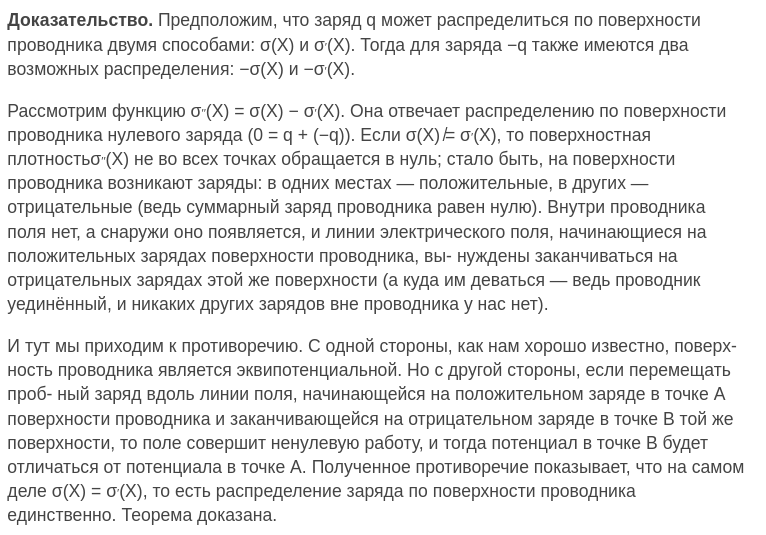
\includegraphics[width=0.7\linewidth]{imgs/q25i1.png}
\end{figure}